\section{Introduction}

\begin{frame}{Quick Questions}
  \large
  \begin{itemize}
    \item How many of you did NOT bring smartphones with you?
    \item How often do you "power off" your smartphone?
    \item Where is your smartphones now?
  \end{itemize}
  \begin{block}{Unique Natures of Smartphones}
    \begin{enumerate}
      \item Carried with you.
      \item Always on.
      \item Mostly idle.
    \end{enumerate}
  \end{block}
  \vspace*{5mm}
  \LARGE \textbf{Ideal} vantage point for network monitoring!
\end{frame}

\begin{frame}{Why "Ideal"?}
  \Large
  \begin{enumerate}
    \item \textbf{Carried with YOU.}
      \begin{itemize}
        \item As opposed to site surveys or statically deployed sniffers.
        \item Capture the \textbf{real user}'s RF conditions and experience.
      \end{itemize}
    \item \textbf{Always on.}
      \begin{itemize}
        \item As opposed to laptops.
        \item Provide \textit{continous} stream of measurements.
      \end{itemize}
    \item \textbf{Mostly Idle.}
      \begin{itemize}
        \item Avoid interrupting normal usage.
      \end{itemize}
    \item \textbf{Additional Benifits.}
      \begin{itemize}
        \item No additional hardware cost.
        \item Easy to deploy (app markets).
      \end{itemize}
  \end{enumerate}
\end{frame}

\begin{frame}{Our Proposal}
  \begin{block}{Use Smartphones to\ldots}
    Long-term large scale network monitoring.
    \begin{itemize}
      \item Network health, performance, etc.
    \end{itemize}
    Short-term local spectrum management.
    \begin{itemize}
      \item Sniff the spectrum on behalf of nearby devices.
      \item Help with channel assignment, rate adaption, etc.
    \end{itemize}
  \end{block}
  \begin{itemize}
    \item {\large\textbf{CANSAS}}\quad {\large \textbf{C}}rowdsourcing {\large
      \textbf{A}}ccess {\large \textbf{N}}etwork {\large \textbf{}S}pectrum
      {\large \textbf{A}}llocation using {\large \textbf{S}}martphones.
    \item {\large\textbf{\PS{}}}\quad Implementing CANSAS on Android smartphones
      for Wifi networks.
  \end{itemize}
\end{frame}

\begin{frame}{\PS{} at a Glance}
  \begin{figure}
    \centering
    \begin{tikzpicture}
      \node[anchor=south west,inner sep=0] at (0,0)
      {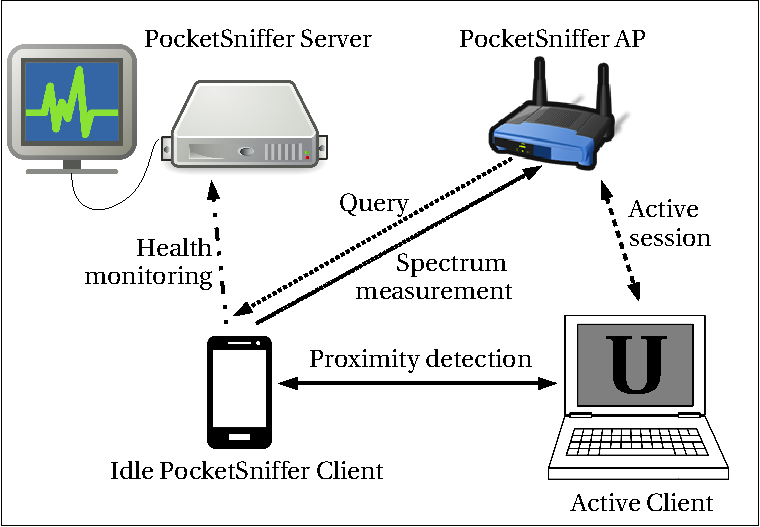
\includegraphics[width=0.6\textwidth]{system-4}};
    \end{tikzpicture}
  \end{figure}
  Long-term large scale network monitoring.
  \begin{itemize}
    \item Network health, performance, etc.
  \end{itemize}
  Short-term local spectrum management.
  \begin{itemize}
    \item Sniff the spectrum on behalf of nearby devices.
    \item Help with channel assignment, rate adaption, etc.
  \end{itemize}
\end{frame}
